\documentclass[final,12pt]{beamer}
%
% load the FAU theme
\usetheme[institute=nat,            % Institute, one of 'fau', 'phil', 'rewi', 'med', 'nat', 'tech'
          logo=art/FAU_DMM_Logo_rgb_10cm    % (optional) provide a project/institution logo instead of seal
         ]{fau-4-3}
\usefonttheme[onlymath]{serif}
%
\usepackage[T1]{fontenc}
\usepackage[utf8]{inputenc}
\usepackage[english]{babel}
\usepackage[babel,english=american]{csquotes} % required for language-specific quotation marks.
\usepackage{graphicx}   % include graphics
\usepackage{lmodern}    % more font sizes
\usepackage{pdfpcnotes}		%notes for pdfpc: use \pnote{}

\usepackage{tikz,pgfplots}
  \pgfplotsset{compat=newest}
  \usetikzlibrary{calc,positioning,spy,arrows.meta}
  % block environment with light blue background, grey outline and rounded corners
  % Usage:
  % \begin{fblock}{<title>}{<width>}
  %    ...
  % \end{fblock}
  \newsavebox\fblockbox
  \newenvironment{fblock}[2]{%
    \begin{lrbox}{\fblockbox}%
      \begin{minipage}{#2\textwidth}%
        \large\ifx#1\empty\else{\color{faublue}#1}\newline\fi
  }{
      \end{minipage}%
    \end{lrbox}%
    \tikz\node[
      fill=faullblue,
      draw=faugrey,
      line width=1pt,
      inner sep=7.5pt,
      rounded corners,
      outer sep=0pt,
    ]{\usebox\fblockbox};%
  }
  % block environment with light blue background, grey outline and rounded corners
  % Usage:
  % \begin{fblock*}{<width>}
  %    ...
  % \end{fblock*}
  \newsavebox\ffblockbox
  \newenvironment{fblock*}[1]{%
    \begin{lrbox}{\ffblockbox}%
      \begin{minipage}{#1\textwidth}%
  }{
      \end{minipage}%
    \end{lrbox}%
    \tikz\node[
      fill=faullblue,
      draw=faugrey,
      line width=1pt,
      inner sep=7.5pt,
      rounded corners,
      outer sep=0pt,
    ]{\usebox\ffblockbox};%
  }
  % block environment with light grey background, grey outline and rounded corners
  % Usage:
  % \begin{gblock}{<title>}{<width>}
  %    ...
  % \end{gblock}
  \newsavebox\gblockbox
  \newenvironment{gblock}[2]{%
    \begin{lrbox}{\gblockbox}%
      \begin{minipage}{#2\textwidth}%
        \large\ifx#1\empty\else{\color{faublue}#1}\newline\fi
  }{
      \end{minipage}%
    \end{lrbox}%
    \tikz\node[
      fill=faullgrey,
      draw=faugrey,
      line width=1pt,
      inner sep=7.5pt,
      rounded corners,
      outer sep=0pt,
    ]{\usebox\gblockbox};%
  }
  % Overlay, useful to connect with arrows or similar
  % Usage:
  % \tikzoverlay at (-1cm,-5cm) {<content>};
  % or
  % \tikzoverlay[text width=5cm] at (-1cm,-5cm) {<content>};
  \tikzset{
    every overlay node/.style={
      anchor=north west, inner sep=0pt,
    },
  }
  \def\tikzoverlay{%
      \tikz[remember picture, overlay]\node[every overlay node]
  }%
  % draw triangulatiom
\newcommand{\triangulation}[1]{
  \pgfmathsetmacro{\triangulationdimension}{#1}
  \pgfmathsetmacro{\triangulationdim}{\triangulationdimension-1}
  \begin{scope}[yscale=-1]
    \draw (1, 1) grid[step=1cm] (\triangulationdimension, \triangulationdimension);
    \foreach \i  in {1,...,\triangulationdim} {
      \foreach \j  in {1,...,\triangulationdim} {
        \draw (\i,\j) -- (\i+1,\j+1);
      }
    }
    \node [below left] at (1,\triangulationdimension) {0,0};
    \node [left] at (1,1) {1,0};
    \node [below] at (\triangulationdimension,\triangulationdimension) {0,1};
    \node [below left] at (2,1) {\(T_1\)};
    \node [above right] at (\triangulationdim,\triangulationdimension) {\(T_K\)};
    \node [below left] at (4,2) {\(T_k\)};
  \end{scope}
}







\DeclareTextFontCommand{\emph}{\mdseries\color{institute}}

\usepackage{dsfont} % double striked symbols
  \newcommand{\IP}{\ensuremath\mathds{P}}
  \newcommand{\IR}{\ensuremath\mathds{R}}
  \newcommand{\IN}{\ensuremath\mathds{N}}
\usepackage{tabularx}             % specify total length of tabular
  \newcolumntype{R}{>{\raggedleft\arraybackslash}X}  \newcolumntype{L}{>{\raggedright\arraybackslash}X}  \newcolumntype{C}{>{\centering\arraybackslash}X}
\usepackage{multirow} % multi-row cells in table
\usepackage{rotating} % write vertically in table
\usepackage{booktabs} % enable \toprule, \midrule, \bottomrule
\usepackage{mathtools}
\usepackage[varg]{txfonts} % provides \varmathbb (for IR, IN, etc), do not load amssymb
\usepackage{amsmath,amssymb}
  \newcommand*{\setT}{\ensuremath{\mathcal{T}}}                    % triangulation
  \newcommand*{\setA}{\ensuremath{\mathcal{A}}}                    % multi-indices
  \newcommand*{\setE}{\ensuremath{\mathcal{E}}}                    % set of edges
  \newcommand*{\setV}{\ensuremath{\mathcal{V}}}                    %
  \newcommand*{\vphi}{\varphi}                                     % basis function
  \newcommand*{\mapEE}{\hat{\vec{\vartheta}}}                      % mapping from ref edge to ref edge
  \renewcommand*{\vec}[1]{{\boldsymbol{#1}}}                       % vector
  \DeclareMathAlphabet{\mathbfsf}{\encodingdefault}{\sfdefault}{bx}{n}
  \newcommand*{\vecc}[1]{\mathbfsf{#1}}                            % tensor or matrix
  \newcommand*{\grad}{\vec{\nabla}}                                % gradient
  \newcommand*{\curl}{\vec{\nabla}\times}                          % curl
  \renewcommand*{\div}{\vec{\nabla}\cdot}                          % divergence
  \newcommand*{\dd}{\mathrm{d}}                                    % differential d for ``int dx''
  \newcommand*{\abs}[1]{\ensuremath{|#1|}}                         % absolute value or volume
  \newcommand*{\card}[1]{\ensuremath{\##1}}                        % cardinality of a set
  \newcommand*{\transpose}[1]{{#1}^\mathrm{T}}                     % transposition
  \newcommand*{\invtrans}[1]{{#1}^\mathrm{-T}}                     % inversion/transposition
  \newcommand*{\jump}[1]{\left\llbracket{#1}\right\rrbracket}      % jump of a discontinuous value
  \DeclareMathOperator*{\diag}{diag}                               % diagonal matrix
  \DeclareMathOperator*{\diam}{diam}                               % diameter
  \DeclareMathOperator*{\sign}{sign}                               % sign
  \newcommand*{\csum}[1]{\sum_{\mathclap{#1}}}
  \newcommand*{\llbrace}{\left\lbrace\!\left\vert}\newcommand*{\rrbrace}{\right\vert\!\right\rbrace}
    \newcommand*{\avg}[1]{\llbrace{#1}\rrbrace}                    % average of a discontinuous value, llbrace, rrbrace is strechable as defined
  %% Roman Numbers %%
  % \newcommand{\I}{I}
  \newcommand{\II}{I\!I}
  \newcommand{\III}{I\!I\!I}
  \newcommand{\IV}{I\!V}
  \newcommand{\V}{V}
  \newcommand{\VI}{V\!I}
  \newcommand{\VII}{V\!I\!I}

\usepackage{textcomp}
\usepackage{listings}
  \definecolor{keywordcolor}{rgb}{0, 0.25, 0.5}
  \definecolor{commentcolor}{rgb}{0.2, 0.5, 0.2}
  \definecolor{stringcolor}{rgb}{0.5, 0.5, 0.2}
  \lstset{language=Matlab,
          frame=tlbr,
          captionpos=t, % caption below the listing
          basicstyle=\ttfamily\large,
          breaklines=false,
          showstringspaces=true,
          stringstyle=\color{stringcolor},
          upquote=true, % to print ' correctly, requires the package textcomp
          commentstyle=\color{commentcolor}\slshape,
          deletekeywords={home, dir},
          keywordstyle=\color{keywordcolor}\bfseries,
          deletekeywords={home, dir, grid},
          morekeywords={blkdiag, case, cat, cd, cell, cell2struct, celldisp, cellplot, char, class, classdef, commandwindow, commandhistory, continue, delete, doc, double, edit, ezplot, factorial, false, filebrowser, fplot, func2str, function_handle, isa, iscell, isequal, islogical, isstruct, logical, ls, methods, mkdir, mldivide, movefile, mrdivide, mtimes, ones, otherwise, parfor, properties, quad, quad2d, repmat, rmdir, spmd, struct,  str2func, struct2cell, switch, true, try, type, execin, getFunctionHandle, main}}

  \newcommand*{\code}[1]{\mbox{\lstinline[basicstyle=\ttfamily\Large]{#1}}}
  \newcommand*{\fatcode}[1]{\mbox{\lstinline[basicstyle=\bfseries\ttfamily\Large]{#1}}}

% Title page
\title[Quadrature-Free LDG]{Master Thesis Introduction:\\[.8em]
  Quadrature-Free Implementation of the Local Discontinuous Garlerkin Method}
\author{Christopher Bross}
\date[2017-02-14]{Erlangen, 2017-02-14}
\institute[AM1,I10]{Applied Mathematics I and Computer Science 10}

\begin{document}

\frame[plain,c]{\titlepage} % plain-Option deaktiviert Kopf- und Fusszeile

\begin{frame}{Outline}
  \tableofcontents
\end{frame}

%        ======================================================
\section{Problem Description and (L)DG Formulation}
%        ======================================================
\begin{frame}
  \frametitle{The Advection Problem}
  \centering%
% MODEL PROBLEM and TRIANGULATION
  \begin{fblock}{Model problem}{0.6}
    Let $J \coloneqq (0,t_\mathrm{end})$ be a finite time interval,
    $\Omega \subset \IR^2$ a polygonally bounded domain with boundary $\partial\Omega$ and outward unit normal $\vec{\nu}$.
    \begin{equation*}
      \begin{aligned}
        \partial_t c(t,\vec{x}) + \div (\vec{u}(t,\vec{x}) c(t,\vec{x}))
        \;&=\; f(t,\vec{x}) \qquad&&\text{in}~J \times \Omega\,, \\
        c \;&= c_\mathrm{D}       &&\text{on}~J \times \partial \Omega_\mathrm{in}(t)\,,\\
        c \;&= c^0                &&\text{on}~\{0\}\times \Omega \,,
      \end{aligned}
    \end{equation*}
    where $\vec{u}: J\times \Omega \rightarrow \IR^2$,
    $f: J\times \Omega\rightarrow \IR$,
    $c^0: \Omega \rightarrow \IR_0^+$,
    $c_\mathrm{D}: J\times\partial\Omega_\mathrm{in}(t) \rightarrow \IR_0^+$,
    $\partial\Omega_\mathrm{in}(t) \coloneqq \{\vec{x}\in\partial\Omega | \vec{u}(t,\vec{x}) \cdot \vec{\nu} < 0\}$.
  \end{fblock}
\end{frame}

\begin{frame}
  \frametitle{Domain decomposition}
  \centering%
  \begin{fblock}{Triangulation and notation}{0.95}
    $\setT_h = \{T\}$ regular family of non-overlapping partitions of $\Omega$ into $K$ closed \emph{triangles $T$} of \emph{characteristic size $h$}, $\overline{\Omega} = \cup T$.
    \emph{$\vec{\nu}_T$} is the exterior \emph{unit normal} on $\partial T$.
    \par
    $\setE = \setE_\Omega \cup \setE_{\partial\Omega} = \{$\emph{$E$}$\}$ are the sets of all \emph{edges}, interior edges, and boundary edges, respectively.
    \par
    \emph{One-sided values} on interior edge $E \in \setE_\Omega$ shared by triangles $T^-$, $T^+$:
    \emph{$w^\pm(\vec{x}) \coloneqq \lim_{\varepsilon\rightarrow 0^+} w(\vec{x} - \varepsilon \vec{\nu}_{T^\pm})$}
  \end{fblock}
  \vfill
  % TODO etwas größer
  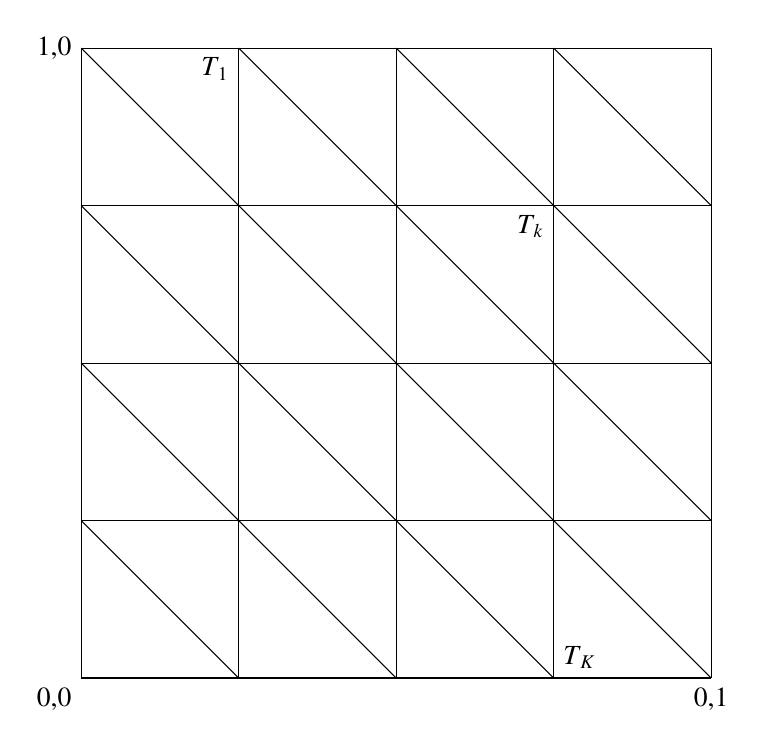
\begin{tikzpicture}[scale=2]
    \triangulation{5}
  \end{tikzpicture}

  Friedrichs-Keller-Triangulation of the unit square.
  \vfill
  \pnote{Genaue NUmerierung noch unklar}
  \pnote{teilen in zwei groe dreiecke dann in die kleinen?}
\end{frame}

% MODEL PROBLEM and TRIANGULATION small
\begin{frame}
  \frametitle{LDG Discretisation}
  \centering%
%% MODEL PROBLEM + TRIANGULATION
  \tikzoverlay (model) at (-5.85cm, 5.55cm) {
    \begin{fblock}{Model problem}{0.2}
      \centering$\partial_t c + \div (\vec{u} c) = f$
    \end{fblock}%
    \begin{minipage}{2.8cm}\centering\Huge
      \emph{$\rightarrow\oplus\leftarrow$}\vspace{1.6cm}
    \end{minipage}%
    \begin{fblock}{Triangulation}{0.2}
      \centering$\setT_h = \{T\}$, $\setE = \{E\}$
    \end{fblock}
  };
%% VARIATIONAL FORMULATION
\only<2>{
  \tikzoverlay (varform) at (-7.91cm, 3cm) {%
    \begin{fblock}{Variational formulation}{0.7}
      Smooth test functions $w: T \rightarrow \IR$, integration by parts over $T\in\setT_h$:
      $$\int_T w \partial_t c(t) \dd\vec{x}
      - \int_T \grad w \cdot \vec{u}(t) c(t) \dd\vec{x}
      + \int_{\partial T} w \vec{u}(t)c(t) \cdot \vec{\nu}_T \dd s
      = \int_T w f(t) \dd\vec{x}$$
    \end{fblock}
  };
  % arrow
  \begin{tikzpicture}[remember picture, overlay]
    \path [line width=1.5pt,->,institute] (model.center) edge (varform.north);
  \end{tikzpicture}
  % notes
  \pnote{wie bei FEM aber rand integral != 0 -> änlich zu FVM}
}\only<3->{}
%% VARIATIONAL FORMULATION small
\only<3->{
  % \tikzoverlay (varform) at (-2.69cm, 3cm) {%
  \tikzoverlay (varform) at (-2.51cm, 3cm) {%
    \begin{fblock}{Variational formulation}{0.21}\end{fblock}
  };
  % arrow
  \begin{tikzpicture}[remember picture, overlay]
    \path [line width=1.5pt,->,institute] (model.center) edge (varform.north);
  \end{tikzpicture}
} \only<1-2>{}
% SEMI-DISCRETE FORMULATION
\only<3>{
  \tikzoverlay (semidisc) at (-11.26cm, 0cm) {%
    \begin{fblock}{Semi-discrete formulation}{0.91}
      With \emph{broken polynomial space} $\IP_p(\setT_h) \;\coloneqq\; \left\{\;w_h : \overline{\Omega}\rightarrow \IR\,;~\forall T\in\setT_h,~ {w_h}|_T\in\IP_p\right\}$
      and $\vec{u}_h \in [\IP_p(\setT_h)]^2$, $f_h(t), c_h^0 \in \IP_p(\setT_h)$,
      \emph{seek $c_h(t) \in \IP_p(\setT_h)$} s.~t. for $t\in J$ and $\forall T^- \in \setT_h, \forall w_h \in \IP_p(\setT_h)$:
      $$\int_{T^-} w_h \partial_t c_h(t) \dd\vec{x}
      - \int_{T^-} \grad w_h \cdot \vec{u}_h(t) c_h(t) \dd\vec{x}
      + \int_{\partial T^-} w_h^- \vec{u}(t) \cdot \vec{\nu}_{T^-} \hat{c}_h(t) \dd s
      = \int_{T^-} w_h f_h(t) \dd\vec{x}\,,$$
      $$\text{where}\quad
      \hat{c}_h(t,\vec{x})\big|_{\partial T^-} = \left\{
      \begin{aligned}
        c_h^-(t,\vec{x})        & \quad\text{if}\quad \vec{u}(t,\vec{x}) \cdot \vec{\nu}_{T^-} \ge 0                                                && \mbox{(outflow from~$T^-$)} \\
        c_h^+(t,\vec{x})        & \quad\text{if}\quad \vec{u}(t,\vec{x}) \cdot \vec{\nu}_{T^-} < 0~\wedge~\vec{x} \notin \partial\Omega_\mathrm{in} && \mbox{(inflow into~$T^-$ from~$T^+$)}\\
        c_\mathrm{D}(t,\vec{x}) & \quad\text{if}\quad  \vec{x} \in \partial\Omega_\mathrm{in}   && \mbox{(inflow into~$T^-$ over~$\partial\Omega_\mathrm{in}$)}
      \end{aligned}\right\}$$
    \end{fblock}
  };
  % arrow
  \begin{tikzpicture}[remember picture, overlay]
    \path [line width=1.5pt,->,institute] (varform.south) edge (semidisc.north);
  \end{tikzpicture}
}\only<2,4->{}
% % SYSTEM OF EQUATIONS
\only<4>{
  \tikzoverlay (system) at (-11.50cm, 0cm) {%
    \begin{fblock}{System of equations}{0.91}
      \emph{Modal DG basis} $\forall k\in\{1,\ldots,K\}$,
      $\IP_p(T_k)=\mathrm{span}\,\big\{ \vphi_{ki} \big\}_{i\in\{1,\ldots,N_p\}}$, where
      $N \coloneqq N_p = (p+1)(p+2)/2$.
      \par
      \emph{Local basis} representation:
      $c_h(t,\vec{x})\big|_{T_k}\eqqcolon \sum_{j=1}^N C_{kj}(t)\,\vphi_{kj}(\vec{x})$,~
      $\vec{u}_h(t,\vec{x})  \big|_{T_k}\eqqcolon \sum_{j=1}^N \sum_{m=1}^2 U_{kj}^m(t)\,\vec{e}_m\vphi_{kj}(\vec{x})\,,$
      $$\begin{multlined}
      \sum_{j=1}^N\partial_t C_{kj}(t)\int_{T_k}\vphi_{ki}\,\vphi_{kj}\,\dd\vec{x}
      -\sum_{j=1}^N C_{kj}(t) \sum_{l=1}^N\sum_{m=1}^2U_{kl}^m(t)\int_{T_k} \partial_{x^m} \vphi_{ki}\,\vphi_{kl}\,\vphi_{kj}\,\dd\vec{x} \\
      + \int_{\partial T_{k^-}} \vphi_{k^-i}\, \Big( \vec{u}(t) \cdot \vec{\nu}_{k^-} \Big)
      \left\{\begin{aligned}
      \scriptstyle
      \sum_{j=1}^N C_{k^-j}(t)\,\vphi_{k^-j}&~~\text{if}~~\vec{u}(t)\cdot\vec{\nu}_{k^-}\ge0 \\
      \scriptstyle
      \sum_{j=1}^N C_{k^+j}(t)\,\vphi_{k^+j}&~~\text{if}~~\vec{u}(t)\cdot\vec{\nu}_{k^-}<0\,\wedge\, \vec{x} \notin \partial\Omega_\mathrm{in} \\
      \scriptstyle
      c_\mathrm{D}(t)                     &~~\text{if}~~ \vec{x} \in \partial\Omega_\mathrm{in}
      \end{aligned}\right\}\,\dd s
      \;=\;
      \sum_{l=1}^N F_{kl}(t) \int_{T_k}\vphi_{ki}\,\vphi_{kl}\,\dd\vec{x}\;,
      \end{multlined}$$
      $$\Leftrightarrow\quad
      \vecc{M}\,\partial_t\vec{C}
      + \left(-\vecc{G}^1 - \vecc{G}^2 + \vecc{R}\right) \vec{C}
      = \vec{L} - \vec{K}_D
      \qquad\Leftrightarrow\quad
      \vecc{M}\,\partial_t\vec{C}(t)+\vecc{A}(t) \vec{C}(t)=\vec{V}(t)$$%
    \end{fblock}
    \pnote{modale basen -> ortogonal zueinander}
  };
  % arrow
  \begin{tikzpicture}[remember picture, overlay]
    \path [line width=1.5pt,->,institute] (varform.south) edge (system.north);
  \end{tikzpicture}
  % command
  \pnote{L2 projetion into polynomial space}
}\only<2-3>{}
\end{frame}


%% KLASISCHER DG ANSATZ
\begin{frame}
  \frametitle{Classical evaluation of the integrals}
  Assemble mass Matrix
  \(\vecc{M}\in\IR^{{KN\times KN}}\):
  \begin{equation*}
    [\vecc{M}]_{(k-1)N+i,(k-1)N+j} \;\coloneqq\; \int_{T_k} \vphi_{ki} \, \vphi_{kj} \, \dd\vec{x}.
  \end{equation*}
  Since $\vphi_{ki}$, $i\in\{1,\ldots,N\}$ have a support only on $T_k$, $\vecc{M}$ has a block diagonal structure
  \begin{equation*}
    \vecc{M} = \begin{bmatrix} \vecc{M}_{T_1} & & \\ & \ddots & \\ & & \vecc{M}_{T_K} \end{bmatrix}
    \qquad\text{with}\qquad
    \vecc{M}_{T_k} \;\coloneqq\; \int_{T_k} \begin{bmatrix}
    \vphi_{k1}\vphi_{k1} & \cdots & \vphi_{k1}\vphi_{kN} \\
    \vdots               & \ddots & \vdots               \\
    \vphi_{kN}\vphi_{k1} & \cdots & \vphi_{kN}\vphi_{kN}
    \end{bmatrix}\,\dd\vec{x}\;.
  \end{equation*}
  Using \emph{(Gaussian) quadrature} for the local mass matrix
  \(\vecc{M}_{T_k}\) the following holds:
  \begin{equation*}
    \begin{split}
      [\vecc{M}_{T_k}]_{i,j}=[\vecc{M}]_{(k-1)N+i,(k-1)N+j} \;
        &\coloneqq\sum_{q=1}^{N_q^{}} \omega_q'\,g_{kij}^{}(x_{kq}')\\
        &\;=\sum_{q=1}^{N_q^{}}\omega_q'\sum_{r=1}^N\phi_{krij}\,\vphi_{kr}(x_{kq}')
    \end{split}
  \end{equation*}
  with \(N_q > N\) the required quadrature points on \(T_k\),
  weightings \(\omega_q'\),
  the polynomial function \(g_{kij}(x)\) and its local basis expansion
  \(\sum_{r=1}^N\phi_{krij}^{}\,\vphi_{kr}^{}(x)\)

  \pnote{Aufwand pro Teilintegral ~ N^2 (Nq>N -> exakt lösen)}
\end{frame}

%% WIE ICH ES MACHEN WERDE
\begin{frame}
\frametitle{Backtransformation to the reference triangle}
  \begin{center}\large
        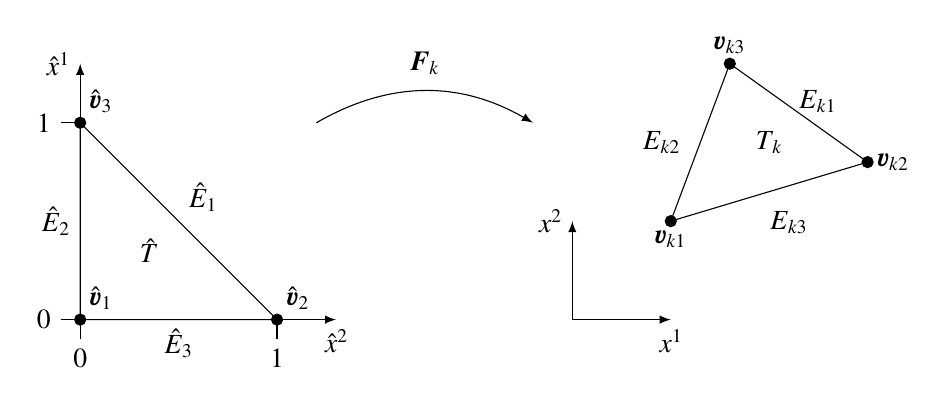
\begin{tikzpicture}[scale=2.5]
      % ref cordinatesystem
      \draw [-latex] (0, -0.1) node[anchor=north]{$0$} -- (0, 1.3) node[anchor=east]{$\hat{x}^1$};
      \draw [-latex] (-0.1, 0) node[anchor=east]{$0$} -- (1.3, 0) node[anchor=north]{$\hat{x}^2$};
      \draw (1, 0) -- (1, -0.1) node[anchor=north] {$1$};
      \draw (0,1) -- (-0.1,1) node[anchor=east] {$1$};

      % ref triangle
      \draw (0, 0) node[inner sep=0pt,outer sep=0pt,draw=black,fill=black,circle,minimum width=4pt] (vhat1) {}
         -- (1, 0) node[inner sep=0pt,outer sep=0pt,draw=black,fill=black,circle,minimum width=4pt] (vhat2) {}
         -- (0, 1) node[inner sep=0pt,outer sep=0pt,draw=black,fill=black,circle,minimum width=4pt] (vhat3) {}
         -- cycle;

      \node at (0.35,0.35) {$\hat{T}$};

      % node labels for ref triangle
      \node[anchor=south west] at (vhat1) {$\hat{\vec{v}}_1$};
      \node[anchor=south west] at (vhat2) {$\hat{\vec{v}}_2$};
      \node[anchor=south west] at (vhat3) {$\hat{\vec{v}}_3$};

      % ref triangl edge labels
      \node[anchor=south west] at (0.5, 0.5) {$\hat{E}_1$};
      \node[anchor=east] at (0, 0.5) {$\hat{E}_2$};
      \node[anchor=north] at (0.5, 0) {$\hat{E}_3$};

      % mapping arrow
      \draw (1.2, 1) edge[-latex,bend left=30] (2.3, 1);
      \node at (1.75, 1.3) {$\vec{F}_k$};

      % physical triangle axis
      \draw[-latex] (2.5, 0) -- (3, 0) node[below] {$x^1$};
      \draw[-latex] (2.5, 0) -- (2.5, 0.5) node[left] {$x^2$};

      % physical triangle
      \draw (3, 0.5)   node[inner sep=0pt,outer sep=0pt,draw=black,fill=black,circle,minimum width=4pt] (vk1) {}
         -- (4, 0.8)   node[inner sep=0pt,outer sep=0pt,draw=black,fill=black,circle,minimum width=4pt] (vk2) {}
         -- (3.3, 1.3) node[inner sep=0pt,outer sep=0pt,draw=black,fill=black,circle,minimum width=4pt] (vk3) {}
         -- cycle;

      \node at (3.5,0.9) {$T_k$};

      % node labels for physical triangle
      \node[anchor=north] at (vk1) {$\vec{v}_{k1}$};
      \node[anchor=west]  at (vk2) {$\vec{v}_{k2}$};
      \node[anchor=south] at (vk3) {$\vec{v}_{k3}$};

      % physical triangle edge labels
      \node[anchor=south west] at (3.6,1.0) {$E_{k1}$};
      \node[anchor=east] at (3.1,0.9) {$E_{k2}$};
      \node[anchor=north] at (3.6,0.6) {$E_{k3}$};
    \end{tikzpicture}
  \end{center}

  Transform reference triangle $\hat{T}$ to physical triangle $T_k$ using an affine mapping
  \begin{equation*}
    \vec{F}_k : \hat{T} \ni \hat{\vec{x}} \mapsto \vecc{B}_k \, \hat{\vec{x}} + \vec{v}_{k1} \in T_k
    \quad\text{with}\quad
    \IR^{2\times2} \ni \vecc{B}_k\coloneqq\Big[ \vec{v}_{k2}-\vec{v}_{k1} \big| \vec{v}_{k3}-\vec{v}_{k1}\Big]\;.
  \end{equation*}
  \vfill
  For $w : \Omega \rightarrow \IR$ we obtain \textbf{transformation formulas}
  \begin{equation*}
    \int_{T_k} w\,(\vec{x})\, \dd \vec{x} \;=\; 2\,|T_k|\int_{\hat{T}} w \circ \vec{F}_k (\hat{\vec{x}})\, \dd \hat{\vec{x}}\;, \qquad
    \int_{E_{kn}} w\,(\vec{x})\, \dd \vec{x} \;=\; \frac{|E_{kn}|}{|\hat{E}_n|}
    \int_{\hat{E}_n} w \circ \vec{F}_k (\hat{\vec{x}})\, \dd \hat{\vec{x}}\;.
  \end{equation*}
\end{frame}

\begin{frame}
  \frametitle{Quadrature free assembly of mass Matrix \(\vecc{M}\)}
  Use simple \emph{monomial basis} \(B_T^{} \equiv \{\phi_{Tr}^{}\}_{r\in 1,\dots ,N_p} %\,|\,0 \leq r \leq N_p\}
  = \{1,\;x,\;y,\;x^2,\;xy,\;y^2,\;\dots\}\)
  to expand polynomials in integrals:
  \begin{equation*}
    \int_{T}P\,\dd\vec{x} = \int_{_T}\sum_{r=1}^Mp_{r}^{}\phi_{Tr}^{}\,\dd\vec{x} = \sum_{r=1}^Mp_{r}^{}\int_T\phi_{Tr}^{}\,\dd\vec{x}
  \end{equation*}
  where \(P\in \IP_p(T)\)% denotes an arbitrary polynomial of degree \(p\)
  , \(M\geq N_p\).
  \vspace*{\fill}

  \pause
  Applied to the block mass matrix \(\vecc{M} \in \IR^{KN\times KN}\):
  \begin{equation*}
    \begin{split}
      [\vecc{M}]_{(k-1)N+i,(k-1)N+j} \;&\coloneqq\; \int_{T_k} \vphi_{ki} \, \vphi_{kj} \, \dd\vec{x}\\
      &\;= 2|T_k| \int_{\hat T}\hat \vphi_i\,\hat \vphi_j\, \dd\vec{\hat x}\\
      &\;= 2|T_k| \sum_{r=1}^{M}p_{ijr}b_r
    \end{split}
  \end{equation*}
  with \emph{analytically precomputed integrals} \(b_r \coloneqq \int_{\hat{T}}\phi_{\hat{T}r}^{}\,\dd\vec{\hat{x}} \).
\end{frame}

\section{Goals of the master thesis}
\begin{frame}
\frametitle{Goals of the master thesis}

\begin{columns}[T]
  \begin{column}{0.45\textwidth}
  \begin{fblock}{from the mathematical viewpoint}{1}
    \begin{itemize}
    \item make use of precomputed integrals of monomials
    \item which combinations of monomials occur?
    \item how to store the pre computed values efficiently?
    \item is it reasonable to neglect higher order monomials?
    \item start with linear advection problem; later non linear problems
      (shallow water eq.)
    \item use FESTUNG to test implementation
    \end{itemize}
  \end{fblock}
  \end{column}
  \begin{column}{0.45\textwidth}
  \pause
  \begin{fblock}{from the computer science viewpoint}{1}
    \begin{itemize}
    \item simple C/C++ code (as baseline for code generation)
    \item 2D triangles on the uniformly refined unit square
    \item assembling the matrix \(\vecc{A}\) for the linear advection problem
    \item later assembling of the vector \(\vec{F-AC}\) for explicit time-stepping
    \item layout of the data structure for precomputed parameters \(p_{ijlr}^m\)
      and integrals \(b_r\)
    \item single core performance
    \end{itemize}
  \end{fblock}
  \end{column}
\end{columns}
\end{frame}

%%%%%%%%%%%%%%%%%%%%%%%%%%%%%%%%%%%%%%%%%%%%%%%%%%%%%%%%%%%%%%%%%%%%%%%%%%%%%%%%
\appendix
\section*{Appendix}

\begin{frame}
  \frametitle{Quadrature free assembly of $\vecc{G^m}$}
  Use simple \emph{monomial basis} \(B_T^{} \equiv \{\phi_{Tr}^{}\}_{r\in 1,\dots ,N_p} %\,|\,0 \leq r \leq N_p\}
  = \{1,\;x,\;y,\;x^2,\;xy,\;y^2,\;\dots\}\)
  to expand polynomials in integrals:
  \begin{equation*}
    \int_{T}P\,\dd\vec{x} = \int_{_T}\sum_{r=1}^Mp_{r}^{}\phi_{Tr}^{}\,\dd\vec{x} = \sum_{r=1}^Mp_{r}^{}\int_T\phi_{Tr}^{}\,\dd\vec{x}
  \end{equation*}
  where \(P\in \IP_p(T)\)% denotes an arbitrary polynomial of degree \(p\)
  , \(M\geq N_p\).
  \vspace*{\fill}

  \pause
  Applied in the block matrix \(\vecc{G}^m \in \IR^{KN\times KN}, m \in \{1,2\}\) from the volume
  integral part:
  \begin{equation*}
    \begin{split}
      [\vecc{G^1}]_{(k-1)N+i,(k-1)N+j} \;&\coloneqq\; \sum_{l=1}^NU_{kl}^1(t)\int_{T_k} \partial_{x^1}\vphi_{ki}\,\vphi_{kl}\,\vphi_{kj}\,\dd\vec{x}\\
      &\;= \sum_{l=1}^NU_{kl}^1(t)\left( \vecc{B}_k^{2,2}\int_{\hat T}\partial_{\hat x^1}\hat \vphi_i\,\hat \vphi_l\,\hat \vphi_j\,\dd\vec{\hat x} - \vecc{B}_k^{2,1}\int_{\hat T}\partial_{\hat x^2}\hat \vphi_i\,\hat \vphi_l\,\hat \vphi_j\,\dd\vec{\hat x} \right)\\
      % &\;= \sum_{l=1}^NU_{kl}^1(t)\left( \vecc{B}_k^{2,2}\sum_{r=1}^Mp_{r,l}^1b_r - \vecc{B}_k^{2,1}\sum_r^Mp_{r,l}^1b_r \right)\\
      % &\;= \sum_{l=1}^NU_{kl}^1(t)\sum_{r=1}^M\left( \vecc{B}_k^{2,2}p_{r,l}^1 - \vecc{B}_k^{2,1}p_{r,l}^1 \right)b_r
      &\;= \sum_{l=1}^NU_{kl}^1(t)\sum_{r=1}^M \beta_{kijlr}^1 b_r
    \end{split}
  \end{equation*}
  with \(\beta_{kijlr}^1 \coloneqq \vecc{B}_k^{2,2}p_{ijlr}^1 - \vecc{B}_k^{2,1}p_{ijlr}^1\)\;
  and \emph{analytically precomputed integrals}
  \(b_r \coloneqq \int_{\hat{T}}\phi_{\hat{T}r}^{}\,\dd\vec{\hat{x}} \).\\
  Analogously for  for \(\vecc{G^2}\).
  % \vspace*{\fill}
\end{frame}

\begin{frame}
\frametitle{Assembly of mass matrix \(\vecc{M}\) in FESTUNG}
  Mass matrix $\vecc{M}\in\IR^{KN\times KN}$:
  \begin{equation*}
    [\vecc{M}]_{(k-1)N+i,(k-1)N+j} \;\coloneqq\; \int_{T_k} \vphi_{ki} \, \vphi_{kj} \, \dd\vec{x}.
  \end{equation*}
  Since $\vphi_{ki}$, $i\in\{1,\ldots,N\}$ have a support only on $T_k$, $\vecc{M}$ has a block diagonal structure
  \begin{equation*}
    \vecc{M} = \begin{bmatrix} \vecc{M}_{T_1} & & \\ & \ddots & \\ & & \vecc{M}_{T_K} \end{bmatrix}
    \qquad\text{with}\qquad
    \vecc{M}_{T_k} \;\coloneqq\; \int_{T_k} \begin{bmatrix}
    \vphi_{k1}\vphi_{k1} & \cdots & \vphi_{k1}\vphi_{kN} \\
    \vdots               & \ddots & \vdots               \\
    \vphi_{kN}\vphi_{k1} & \cdots & \vphi_{kN}\vphi_{kN}
    \end{bmatrix}\,\dd\vec{x}\;.
  \end{equation*}
  For the local mass matrix holds
  \begin{equation*}
    \vecc{M}_{T_k} \;=\; 2\,|T_k|\,\hat{\vecc{M}}
    \qquad\text{with}\qquad
    \hat{\vecc{M}} \;\coloneqq\; \int_{\hat{T}} \begin{bmatrix}
    \hat{\vphi}_{1}\hat{\vphi}_{1} & \cdots & \hat{\vphi}_{1}\hat{\vphi}_{N} \\
    \vdots                         & \ddots & \vdots                         \\
    \hat{\vphi}_{N}\hat{\vphi}_{1} & \cdots & \hat{\vphi}_{N}\hat{\vphi}_{N}
    \end{bmatrix}\,\dd\vec{x}
  \end{equation*}
  and $\hat{\vphi}_i(\hat{\vec{x}}) = \vphi_{ki} \circ \vec{F}_k (\hat{\vec{x}})$.
  Hence, the global mass matrix $\vecc{M}$ can be expressed as
  \begin{equation*}
    \vecc{M} \;=\;
    \begin{bmatrix} \vecc{M}_{T_1} & & \\ & \ddots & \\ & & \vecc{M}_{T_K} \end{bmatrix}
    \; = \; 2 \, \begin{bmatrix} |T_1| & & \\ & \ddots & \\ & & |T_k| \end{bmatrix}
    \otimes \hat{\vecc{M}}\;,
  \end{equation*}
  where $\otimes$ denotes the Kronecker product.
\end{frame}

\begin{frame}
\frametitle{L2-projection of coefficient functions}
  We assumed $d_h(t), f_h(t), c_h^0 \in \IP_p(\setT_h)$.

  Given an algebraic expression, e.\,g., for $d$ and seek the representation matrix $\vecc{D}(t) \in \IR^{K\times K}$ such that
  \begin{equation*}
    d_h(t,\vec{x})\big|_{T_k} = \sum_{j=1}^N D_{kj}(t)\, \vphi_{kj}(\vec{x})\;.
  \end{equation*}

  Produce $d_h$ using the \textbf{$L^2$ projection} defined locally for $T_k \in \setT_h$ by
  \begin{equation*}
    \forall w_h \in \IP_d(T)\,, \quad \int_{T_k} w_h\, d_h(t) = \int_{T_k} w_h\, d(t)\;.
  \end{equation*}
\end{frame}

\begin{frame}
\frametitle{Time discretization}
  The linear system can be written as
  \begin{equation*}
    \vecc{M}\partial_t \vec{C}(t) = \vec{V}(t) - \vecc{A}(t) \vec{C}(t) \eqqcolon \vec{S}(t, \vec{C}(t))\,.
  \end{equation*}
  Discretize in time using \emph{TVD Runge--Kutta methods}\footnote{S. Gottlieb, C.-W. Shu, Strong stability-preserving high-order time discretization methods, Math. Comp. 67 (221) (1998) 73–85. doi:10.1090/S0025-5718-98-00913-2} (SSP Runge--Kutta) of orders \emph{$s \in \{1,2,3\}$}.
  \par
  Let $0 = t^1 < t^2 < \ldots t_\mathrm{end}$, $\Delta t^n = t^{n+1} - t^n$,
  $\vec{C}^n \coloneqq \vec{C}(t^n)$, and
  $\vec{S}^{n+\delta_i} \coloneqq \vec{S}(t^n+\delta_i\Delta t^n)$.
  \begin{equation*}
    \begin{array}{lll}
    \vec{C}^{(0)} &=\; \vec{C}^{n} \,, \\
    \vec{C}^{(i)} &=\; \omega_i\,\vec{C}^{n} + (1-\omega_i)\,\left( \vec{C}^{(i-1)}
    + \Delta t^n\,\vecc{M}^{-1} \vec{S}^{n + \delta_i} \right) \,, \quad \text{for}~i = 1,\ldots,s\,,\\
    \vec{C}^{n+1} &=\; \vec{C}^{(s)} \,.
    \end{array}
  \end{equation*}
  When possible, choose $s = p+1$.
\end{frame}

\end{document}
